\documentclass{article}
\usepackage{minted}
\usepackage{graphicx}
\usepackage{listings}
\usepackage{courier}
\setminted[python]{fontfamily=courier}

\begin{document}
\section{UML diagram}
The following diagram shows all the classes of this application, and their relations with both one another and the problem domain classes.
\begin{figure}[ht]
  \begin{center}
    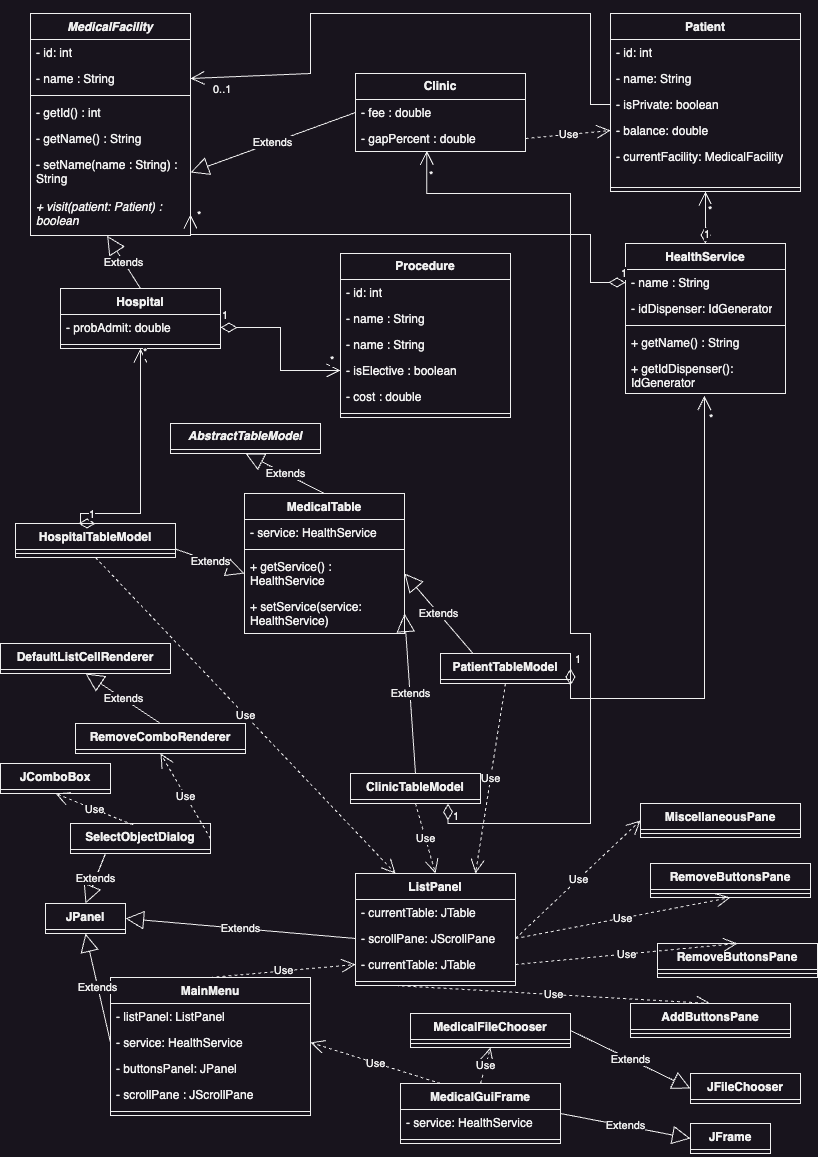
\includegraphics[width=0.95\textwidth]{figures/UML_diagram.png}
  \end{center}
\end{figure}

\section{Source code}%
\label{sec:source_code}
The source code for this assignment can be found below, and it is divided in sections like so:
\begin{itemize}
  \item Components
  \item Models
\end{itemize}

\subsection{Components}\label{subsec:components} % (fold)
\textit{MedicalGui.java}
\inputminted{java}{./src/main/java/com/yvesstraten/medicalconsolegui/MedicalGui.java}

\textit{MainMenu.java}
\inputminted{java}{./src/main/java/com/yvesstraten/medicalconsolegui/components/MainMenu.java}

\textit{MedicalGuiFrame.java}
\inputminted{java}{./src/main/java/com/yvesstraten/medicalconsolegui/components/MedicalGuiFrame.java}

\textit{AddButtonsPane.java}
\inputminted{java}{./src/main/java/com/yvesstraten/medicalconsolegui/components/AddButtonsPane.java}

\textit{MiscellaneousPane.java}
\inputminted{java}{./src/main/java/com/yvesstraten/medicalconsolegui/components/MiscellaneousPane.java}

\textit{RemoveComboRenderer.java}
\inputminted{java}{./src/main/java/com/yvesstraten/medicalconsolegui/RemoveComboRenderer.java}

\textit{RemoveButtonsPane.java}
\inputminted{java}{./src/main/java/com/yvesstraten/medicalconsolegui/components/RemoveButtonsPane.java}

\textit{MedicalFileChooser.java}
\inputminted{java}{./src/main/java/com/yvesstraten/medicalconsolegui/components/MedicalFileChooser.java}

\textit{SelectObjectDialog.java}
\inputminted{java}{./src/main/java/com/yvesstraten/medicalconsolegui/components/SelectObjectDialog.java}

\textit{ListPanel.java}
\inputminted{java}{./src/main/java/com/yvesstraten/medicalconsolegui/components/ListPanel.java}
% subsection Components (end)

\subsection{Models}\label{sec:models} % (fold)
\textit{ProcedureTableModel.java}
\inputminted{java}{./src/main/java/com/yvesstraten/medicalconsolegui/models/ProcedureTableModel.java}

\textit{MedicalTableModel.java}
\inputminted{java}{./src/main/java/com/yvesstraten/medicalconsolegui/models/MedicalTableModel.java}


\textit{FacilityTableModel.java}
\inputminted{java}{./src/main/java/com/yvesstraten/medicalconsolegui/models/FacilityTableModel.java}

\textit{HospitalTableModel.java}
\inputminted{java}{./src/main/java/com/yvesstraten/medicalconsolegui/models/HospitalTableModel.java}

\textit{PatientTableModel.java}
\inputminted{java}{./src/main/java/com/yvesstraten/medicalconsolegui/models/PatientTableModel.java}

\textit{ClinicTableModel.java}
\inputminted{java}{./src/main/java/com/yvesstraten/medicalconsolegui/models/ClinicTableModel.java}
% subsection Models (end)

\section{Runtime output}\label{sec:runtime_output} % (fold)
Several tests were undertaken to ensure that this application works as intended.

% section Runtime output (end)

\end{document}
